% flashcards-title: Rod lying mid-scale along a millimeter ruler
% flashcards-desc: A shaded metal rod lies just above a ruler scale whose labeled marks run from two to eight centimeters, with ten small millimeter steps between neighboring labels. The rod's left end aligns with the labeled 2 mark and its right end lies between the labeled 7 and 8 marks, four small steps past the 7. Faint dashed guides drop from each rod end to the scale.
\documentclass[dvisvgm,tikz,border=8pt]{standalone}
\usepackage{tikz}
\usetikzlibrary{arrows.meta,calc,positioning}
\definecolor{DeckInk}{HTML}{172A3A}
\definecolor{DeckAccent}{HTML}{176B87}
\definecolor{DeckWarm}{HTML}{D97706}
\definecolor{DeckMuted}{HTML}{667784}
\definecolor{DeckPaper}{HTML}{F7FAFC}
\tikzset{
  every node/.style={font=\sffamily, text=DeckInk},
  object/.style={draw=DeckInk, line width=1.1pt, fill=DeckPaper},
  primary/.style={draw=DeckAccent, line width=1.5pt},
  boundary/.style={draw=DeckAccent, line width=1.5pt, dashed, rounded corners=6pt},
  guide/.style={draw=DeckMuted, line width=0.9pt, dashed},
  dimension/.style={{Stealth[length=3.2mm,width=2.2mm]}-{Stealth[length=3.2mm,width=2.2mm]}, draw=DeckWarm, line width=1.2pt},
  motion/.style={-{Stealth[length=3.5mm,width=2.5mm]}, draw=DeckAccent, line width=1.5pt, dashed},
}

\begin{document}
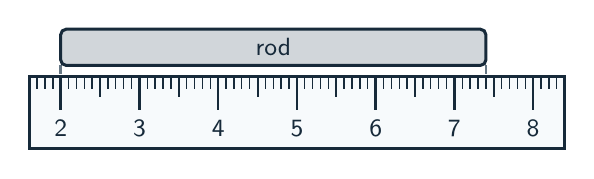
\begin{tikzpicture}[x=1cm,y=1cm]
  % Ruler body
  \draw[object] (1.6,0.08) rectangle (8.4,1.0);
  % Millimeter ticks
  \foreach \x in {1.6,1.7,...,8.35}
    \draw[DeckInk, line width=0.5pt] (\x,1.0) -- (\x,0.84);
  % Half-centimeter ticks
  \foreach \x in {2.5,3.5,...,7.5}
    \draw[DeckInk, line width=0.7pt] (\x,1.0) -- (\x,0.74);
  % Centimeter ticks and labels
  \foreach \x in {2,...,8}{
    \draw[DeckInk, line width=0.9pt] (\x,1.0) -- (\x,0.58);
    \node[font=\sffamily\small] at (\x,0.34) {\x};
  }
  % Guides from rod ends to the scale, painted before the rod
  \draw[guide] (2.0,1.14) -- (2.0,1.0);
  \draw[guide] (7.4,1.14) -- (7.4,1.0);
  % Rod with ends at 2.0 and 7.4
  \draw[draw=DeckInk, line width=1.1pt, fill=DeckMuted!30, rounded corners=2pt]
    (2.0,1.14) rectangle (7.4,1.6);
  \node[font=\sffamily\small] at (4.7,1.37) {rod};
\end{tikzpicture}
\end{document}
